\chapter{Árvore binária de busca }

Uma árvore binária de busca é uma estrutura de dados de árvore binária enraizada tal que para cada nó interno da árvore armazena uma chave maior que todos os nós da esquerda e menor que os todos os nós da direita. Como um mesmo conjunto de valores de chaves podemos construir várias árvore de busca binária. No exemplo abaixo, temos duas árvore de busca binária formada pelos valores de chaves \{5,10,12,15,20,25\}:

\includegraphics[width=.6\textwidth]{images/9-5.png}

Uma árvore binária de busca com $n$ nós pode ter uma altura h variando entre  $ \lceil log~ (n+1)  \rceil \leq h \leq n$.

Nessa estrutura de dados, a complexidade de tempo para realizar as operações de busca, inserção e remoção são proporcionais a altura da árvore. Por isso, estamos interessados em trabalhar com uma árvore de busca com a altura próxima de $log~ n$. No exemplo acima, as operações de busca, inserção e remoção são mais demorado na árvore binária de busca da direita do que na esquerda. Contudo, as alturas das duas árvores estão próximas de $log ~n$. O nosso primeiro problema será construir uma árvore binária de busca com uma altura próxima $log~ n$ a partir de um conjunto de chaves.

Inicialmente, vamos realizar uma ordenação do nosso conjunto de chaves. 

\begin{minted}
[
frame=lines,
bgcolor=LightGray,
fontsize=\footnotesize,
linenos
]
{C++}
template <typename T> 
NodeTree<T>* createCompleteTree(vector <T> keys){
    sort(keys.begin(), keys.end() );
    return createCompleteTreeAux(keys);
}
\end{minted}


Durante o processo de criação da nossa árvore binária de busca, escolheremos o elemento do meio como raiz da nossa árvore de busca. Em seguida, as chaves $keys[0..mid-1]$ serão usadas para criar a subárvore da esquerda e as chaves $keys[mid+1, keys.size()-1]$ serão usadas para criar a subárvore da direita.

\begin{minted}
[
frame=lines,
bgcolor=LightGray,
fontsize=\footnotesize,
linenos
]
{C++}

template <typename T> 
NodeTree<T>* createCompleteTreeAux(vector <T> keys){
    int n = keys.size();
    if(n == 0){
        return nullptr;
    }else if(n == 1){
        return  new NodeTree<T>( keys[0] );
    }else{
        int mid = n/2;

        NodeTree<T>* root = new NodeTree<T>( keys[mid] );

        vector <T> leftkeys;
        vector <T> rightkeys;

        leftkeys.assign( keys.begin(), keys.begin() + mid);
        rightkeys.assign( keys.begin() + mid + 1, keys.end() );

        root->left  = createCompleteTreeAux(leftkeys);
        root->right = createCompleteTreeAux(rightkeys);

        return root;
    }
}
\end{minted}

Dessa maneira, conseguimos construir uma árvore de busca com a complexidade de tempo $O(n~ log~ n)$.

A operação de busca em um árvore binária de busca pode tirar proveito da estrutura da árvore binária de busca para realizar uma busca baseada no mesmo princípio da busca binária.

\begin{minted}
[
frame=lines,
bgcolor=LightGray,
fontsize=\footnotesize,
linenos
]
{C++}
template <typename T> 
NodeTree<T> * search(NodeTree<T> * root, T key){
    if(root == nullptr)
        return nullptr;
    else{
        if( root->key == key )
            return root;
        else if( key < root->key)
            return search(root->left, key);
        else 
            return search(root->right, key);
    }
}
\end{minted}

Note que se a nossa chave de busca (key) for menor que a chave da raiz da árvore (root->key) então o nó contendo a chave key (se ela existir) estará na subárvore da esquerda. Se a chave for maior que a chave da raiz da árvore, então o nó com essa chave deve estar na subárvore da direita.

A operação de inserção na árvore de busca segue uma idéia semelhante do processo de busca contudo o algoritmo de inserção apresentado não é capaz de manter a altura da árvore no seu valor mínimo.


\begin{minted}
[
frame=lines,
bgcolor=LightGray,
fontsize=\footnotesize,
linenos
]
{C++}
template <typename T> 
template <typename T> 
NodeTree<T>* insert(NodeTree<T> * root, T key){
    if(root == nullptr)
        return new NodeTree<T>(key);
    else{
        if( key < root->key ){
            root->left = insert(root->left, key);
        }else{
            root->right = insert(root->right, key);
        }
        return root;
    }
}
\end{minted}

Considere a seguinte árvore construída com o seguinte conjunto de chaves \{4,6,7,2,3,10,12,9,-5, 8\} utilizando o algoritmo acima:

\begin{figure}
    \centering
    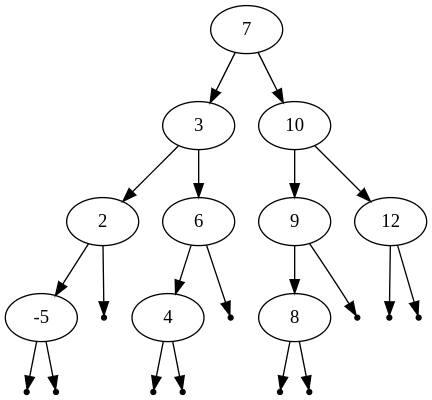
\includegraphics[scale=0.5]{images/bst.png}

    \caption{Árvore binária de busca formada pelas chaves \{4,6,7,2,3,10,12,9,-5, 8\} }
    \label{fig::bst1}
\end{figure}

Se você inserir as chaves {-4,-3}, aumentaremos a altura da árvore em duas unidades.

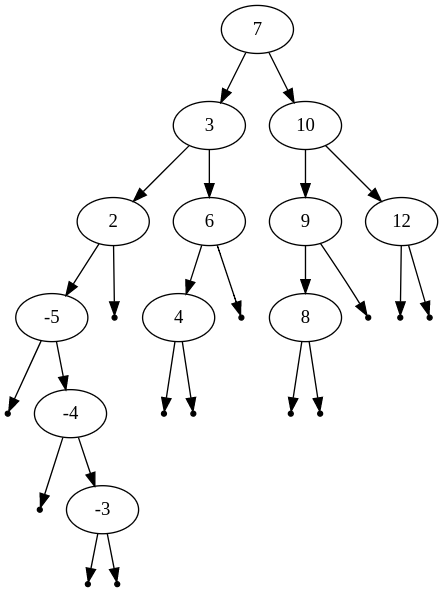
\includegraphics[scale=0.5]{images/bst2.png}

Esse problema será resolvido desenvolvendo uma função de inserção na árvore de busca capaz de manter a altura da árvore em  $O(log ~n)$

A operação de remoção em uma árvore binária de busca pode ser realizada da seguinte maneira:

\begin{enumerate}
    \item Primeiramente, encontraremos o nó raiz da subárvore (node) que será alterada.
    \begin{enumerate}
    \item Se node->right for nullptr, então salvamos o node->left em q, deletamos node e devolvemos q. Note que se  node->left for nullptr então significa que node não tem filhos e que node pode ser simplesmente removida e árvore resultante é vazia. Se node->left for diferente de nullptr, então node->left será a raiz da árvore resultante da remoção de node.
    \item Se node->right for diferente de nullptr, precisamos encontrar o sucessor de node e o seu pai para encontrar a árvore resultante da remoção de node. O nó sucessor será o nó com o menor valor da subárvore da direita. O nó com o menor valor será o nó que está mais à esquerda da subárvore da direita. Na Figura \ref{fig::bst1}, o sucessor do nó com chave 7 é o nó com chave 8 que é o nó mais à esquerda da subárvore da direita do nó com chave 7.
    
    
    Temos que considerar dois novos casos:
        \begin{enumerate}
        \item Se o nó pai do sucessor for igual ao nó a ser removido, então precisamos colocar o nó sucessor como raiz da árvore resultante da remoção de node e a esquerda do nó sucessor será ajustada para a esquerda do nó a ser removido.
        \item Se o nó pai do sucessor for diferente ao nó a ser removido, ajustaremos a esquerda do nó pai para a direita do nó sucessor. Em seguida, colocaremos o nó sucessor como raiz da subárvore resultante da remoção de nó node.
        
        \end{enumerate}
        
    \end{enumerate}
\end{enumerate}

O código que reflete a ideia acima é o seguinte:

\begin{minted}
[
frame=lines,
bgcolor=LightGray,
fontsize=\footnotesize,
linenos
]
{C++}
template <typename T> 
NodeTree<T> * removeRoot(NodeTree<T> * node){

    if( node->right == nullptr){
        NodeTree<T> * q = node->left;
        delete node;
        return q;
    }else{
        
        NodeTree<T> * pai  = node; 
        NodeTree<T> * succ = node->right;

        while( succ->left != nullptr){
            pai = succ;
            succ = succ->left;
        }

        if( pai == node ){
            succ->left = node->left;
            delete node;
            return succ;
        }else{
            pai->left = succ->right;
            succ->right = node->right;
            succ->left  = node->left;
            delete node;
            return succ;
        }
        
    }
}

template <typename T> 
NodeTree<T> * remove(NodeTree<T> * root, T key){
    
    if(root == nullptr)
        return nullptr;
    else if( root->key == key ){
        return removeRoot(root);
    }else if( key < root->key ){
        root->left = remove(root->left, key);
    }else {
        root->right = remove(root->right, key);
    }
    return root;
}
\end{minted}

Podemos adicionar o campo size a nossa NodeTree e garantir que as operações de inserção e remoção da árvore mantenham esse campo bem calculado.

\begin{minted}
[
frame=lines,
bgcolor=LightGray,
fontsize=\footnotesize,
linenos
]
{C++}
template <typename T> 
NodeTree<T>* insert(NodeTree<T> * root, T key){
    if(root == nullptr)
        return new NodeTree<T>(key);
    else{
        if( key < root->key ){
            root->left = insert(root->left, key);
            root->size++;
        }else{
            root->right = insert(root->right, key);
            root->size++;
        }
        return root;
    }
}
\end{minted}

O mesmo pode ser realizado na função remove:

\begin{minted}
[
frame=lines,
bgcolor=LightGray,
fontsize=\footnotesize,
linenos
]
{C++}

template <typename T> 
NodeTree<T> * remove(NodeTree<T> * root, T key){
    
    if(root == nullptr)
        return nullptr;
    else if( root->key == key ){
        return removeRoot(root);
    }else if( key < root->key ){
        root->left = remove(root->left, key);
        root->size--;
    }else {
        root->right = remove(root->right, key);
        root->size--;
    }
    return root;
}
\end{minted}

As alterações que devem ser realizadas na função removeRoot serão deixadas para o leitor.


